\documentclass[12pt]{article}%
\usepackage{amsfonts}
\usepackage{fancyhdr}
\usepackage{comment}
\usepackage[a4paper, top=2.5cm, bottom=2.5cm, left=2.2cm, right=2.2cm]%
{geometry}
\usepackage{times}
\usepackage{amsmath}
\usepackage{subcaption}
\usepackage{changepage}
\usepackage{stmaryrd}
\usepackage{amssymb}
\usepackage{graphicx}
\usepackage{float}
\usepackage{caption}
\usepackage{hyperref}


\begin{document}

\title{Logo detection in a video}
\author{Benoit Audigier}
\date{\today}



\maketitle
\section{Introduction}

\paragraph{}
The aim of the project is to find logos of a Sysnav company in a video. Deep learning and computer vision are used for this matter.

\begin{figure}[H]
\centering

\includegraphics[width=.2\textwidth]{images/logo.png}
\caption{\label{fig:logo}Sysnav logo}
\end{figure}




\section{First Approach}

\paragraph{}
The first approach consists in using computer vision with the very specific shape of the logo. To that extent, an edge detection using the OpenCV library is used. Every frame is converted in black and white, blurred and the gradient of the intensity of the pixel is analyzed to detect the edges. The Canny Edge Detection \cite{canny} implemented by OpenCV is used. 

\paragraph{}
However, the level of maxVal and minVal are not that easy to determine.  Those two values represent the thresholds that determine if the gradient is high enough or not high enough to be an edge. If the value is in between, the connectivity is taken into account. Indeed, the distribution of the gradient really depends on the images of the video, very different following the movement of the camera. That's why no efficient way of calibrating these values was determined; the images are often way too blurry because of the movement of the camera or the bad luminosity (see \ref{fig:edgeDetection}). Calibrating the values on the level of luminosity of the image was not efficient: the distribution was too different from one frame to another to correctly detect the edges - especially on the blurry images.

\captionsetup[subfigure]{labelformat=simple, labelsep=period}
\begin{figure}
	\centering
	\begin{subfigure}[t]{5cm}
		\centering
		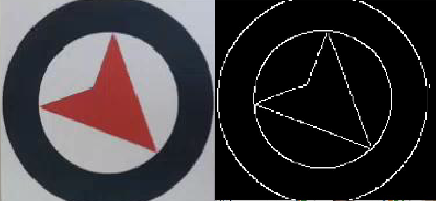
\includegraphics[width=4.5cm]{images/edgeDetect1.png}
		\caption{The edges are clear, shapes are easy to detect.}
	\end{subfigure}
	\begin{subfigure}[t]{5cm}
		\centering
		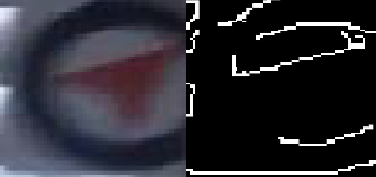
\includegraphics[width=4.5cm]{images/edgeDetect2.png}
		\caption{The edges less clear, the background interferes}
	\end{subfigure}
	\begin{subfigure}[t]{5cm}
		\centering
		
\includegraphics[width=4.5cm]{images/edgeDetect3.png}
		\caption{The edges are too blurry, the quality is not good enough, shapes are not perceptible.}
	\end{subfigure}
	\caption{Edge detection on several crops of images more or less blurred and small with the same thresholds.}\label{fig:edgeDetection}
\end{figure}

\paragraph{}
Detecting the circles inside the picture reveals to be too difficult to calibrate; a first focus on where to look before using computer vision is required for proper results. To that extent, deep learning is used.

\section{Deep learning}

\paragraph{}
The deep learning approach relies on the use of a neural network already trained and adapted from the ImageNet and COCO classification problem, as described in the documentation of \href{https://github.com/tensorflow/models/tree/master/research/object_detection}{Google's Object Detection API} \cite{googleAPI}.
The idea is to retrain it with the local problem of our logo detection, and apply it frame by frame to detect boxes where the logo is likely to be.

\paragraph{}
The pros of that method is that it doesn't rely exactly on edge detection; it's more subtle, the features extracted from the frames are more diverse and more elaborate. It would also be adaptable to any object recognition, not only the logo problem, and this quite easily.

\paragraph{}
The cons are the fact that the model is very hard to explain; it's not trivial to determine why a box has been selected and one has not. This is a recurring problem with deep learning, even though a recent article on random forest applied to meta level training dataset is giving clues on interpretability  of hidden layers of a Deep CNN network \cite{interpretability}. Furthermore, the computation is bigger than with a simple edge detection. The training part can also be problematic; this model has been trained during 12 hours on a CPU but could give better results with a lower training rate/more computation power (no GPU available here).



\subsection{Dataset}

\subsubsection{Data augmentation}

\paragraph{}
The first thing to consider is the fact that a dataset to train the neural network. For this, data augmentation is used. A short video pretty clear of the logo is first shot, in order to have labeled frames zoomed on the logo. Then, several methods are used to have a dataset as diverse as possible. The dataset is not modified directly, but on the fly. The images, when regrouped in batches are applied some random transformation. The efficiency of simple techniques such as the one described in the section are still quite efficient and relevant \cite{dataAugmentation} 

\paragraph{}
By using enough batches, we can make sure that the probability of using all the possible combinations is pretty high. For example, if we apply $2$ transformation, let's call $A_i$ the event "the possibility i did not happen", $\forall i \in \llbracket 1~;~ n \rrbracket$ (with our configuration, there are only $n = 4$ possibilities). We denote $p_i$ the probability of $A_i$ (with our configuration, if we use the same probability $q = .5$, we have $\forall i \in \llbracket 1~;~ n \rrbracket, \ p_i = .75$). Then, for a batch of size $m$ we can the probability of not having used all the possibilities:
\begin{align*}
\Pr(\cap_{i=1}^{n} \overline{A_i}) &= 1 - \Pr(\cup_{i=1}^{n} A_{i})\\
&\geq 1 - \sum_{i=1}^{n} \Pr(A_i) \\
&\geq 1 - \sum_{i=1}^{n} p_i^{m} \\
\end{align*}
which is around $98\%$ for $m=20$ in this example. This is of course a simplistic situation. In the real use, the number of batch is very high compared to the value of each $p_i$, enough for this probability to remain in the same area - and be sure that the data augmentation was entirely exploited.

The transformations (see \ref{fig:dataAugmentationSample}) are used to make sure that the neural network has seen as many real life cases as possible. Here are what is used:
\begin{itemize}
    \item Random crops. The new image must remain big enough to have most of the logo on the frame. This simulates the logos that are partially cropped in the video.
    \item Random blurs. This simulates the movements of the camera.
    \item Random luminosity adjustments (brighter and darker).
    \item Random rotations, random horizontal and vertical flips.
    \item Random resizing.
\end{itemize}




\captionsetup[subfigure]{labelformat=simple, labelsep=period}
\begin{figure}
	\centering
	\begin{subfigure}[t]{2.5cm}
		\centering
		
\includegraphics[width=2.5cm]{images/logo.png}
		\caption{Original}
	\end{subfigure}
	\begin{subfigure}[t]{2.5cm}
		\centering
		
\includegraphics[width=2.5cm]{images/logoRandomRotation.png}
		\caption{Rotation}
	\end{subfigure}
	\begin{subfigure}[t]{2.5cm}
		\centering
		
\includegraphics[width=2.5cm]{images/logoLuminosity.png}
		\caption{Luminosity}
	\end{subfigure}
	\begin{subfigure}[t]{2.5cm}
		\centering
		
\includegraphics[width=2.5cm]{images/logoBlurred.png}
		\caption{Blurred}
	\end{subfigure}
	\begin{subfigure}[t]{2.5cm}
		\centering
		
\includegraphics[width=2.5cm]{images/logoRandomCrop.png}
		\caption{Cropped}
	\end{subfigure}
	\caption{Different transformations. They are not combined in this sample, which is the case in reality during the training.}\label{fig:dataAugmentationSample}
\end{figure}

\subsubsection{Train, validation and test set}

\paragraph{}
The dataset is then separated between a training set (70\%), a validation test(20\%) and a test set (10\%). The later is not touch during any part of the training, and used to judge the performances after training to make sure we're not overfitting. We move then forward to the training phase.

\subsection{Training}

\paragraph{}
The neural network used is a NaSNet architecture \cite{nasnet}. All the layers but the latest one is frozen, and the last one is replaced by a dense layer with one category output with a sigmoid activation function and a $.5$ threshold. Weight decay ($0.9$) is added to avoid overfitting; no dropout is used. A Nadam optimizer (Adam with a momentum component \cite{nadam}), with a learning rate at $0.001$, and a constant for numerical stability $\epsilon = 1$.

\paragraph{}
The training phase is performed on a CPU for 12 hours. This is definitely not optimal. A smaller or decreasing learning rate could give better results but requires too much computer power. The parameters could have been optimized in a better way but due to time and computation power constraint, the values of the literature have been used.

\begin{figure}
\centering
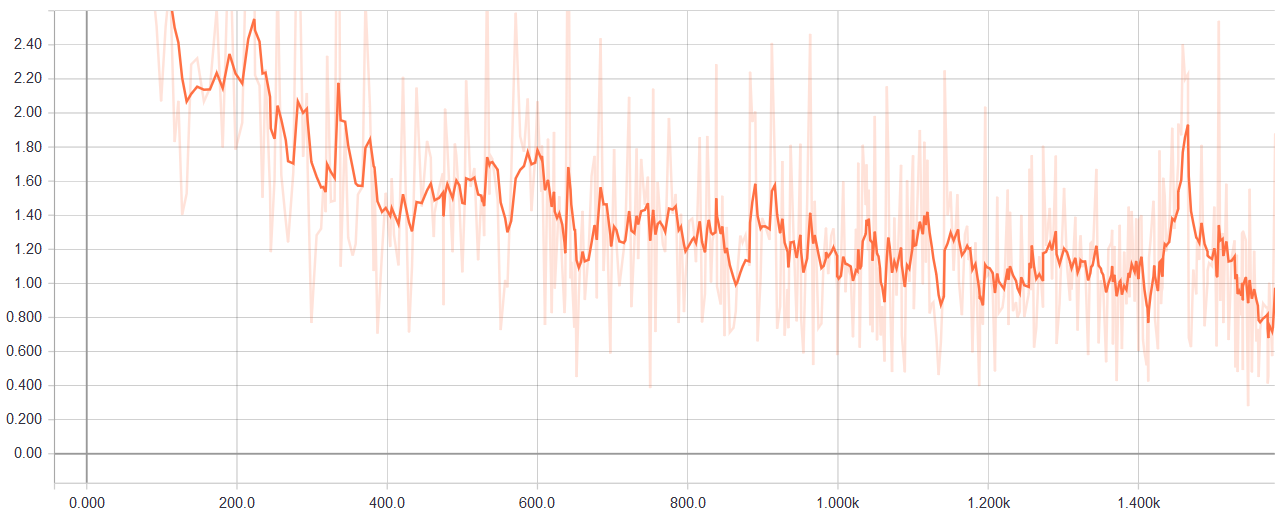
\includegraphics[width=15cm]{images/lossCurve.PNG}
\caption{\label{fig:loss}Loss evolution during the training. We can see that the training is not complete yet after less than 2,000 epochs.}
\end{figure}

\subsubsection{Results}

\paragraph{}
The results from this methods are mixed. With this learning rate, we barely reach a loss below 1 (see \ref{fig:loss}), and the training could be ran for more epochs (around 10,000 would be better). That said, it performs better than the simple edge/circle detection previously used (see \ref{fig:predictionResult}). It seems not to be that much bothered by the blurriness/bad luminosity of a few frames. There are however too many false positive that need to be reduced using another independent method. This is why another filter is added to the process.

\captionsetup[subfigure]{labelformat=simple, labelsep=period}
\begin{figure}
	\centering
	\begin{subfigure}[t]{4cm}
		\centering
		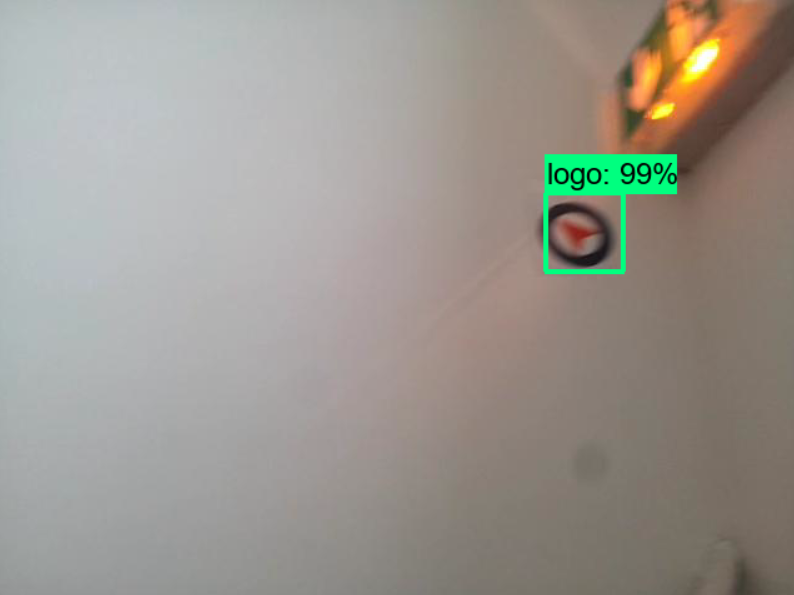
\includegraphics[width=4cm]{images/detection1.PNG}
	\end{subfigure}
	\begin{subfigure}[t]{4cm}
		\centering
		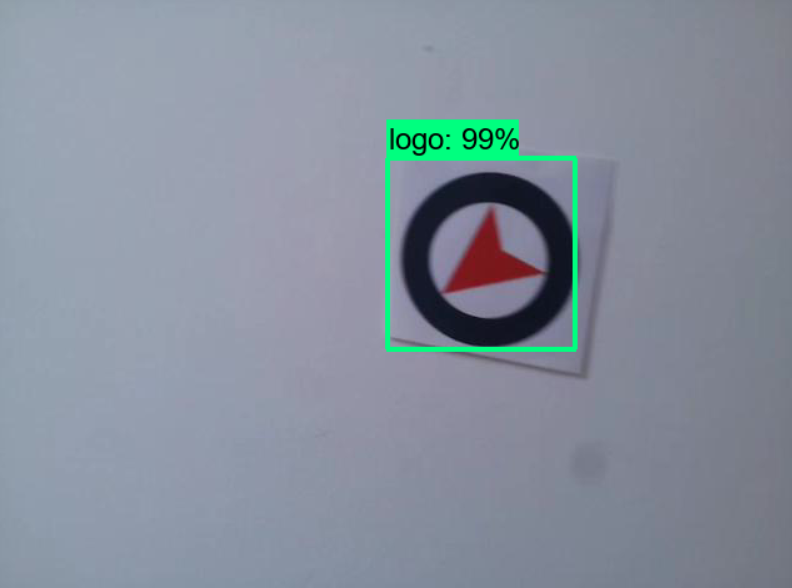
\includegraphics[width=4cm]{images/detection2.PNG}
	\end{subfigure}
	\begin{subfigure}[t]{4cm}
		\centering
		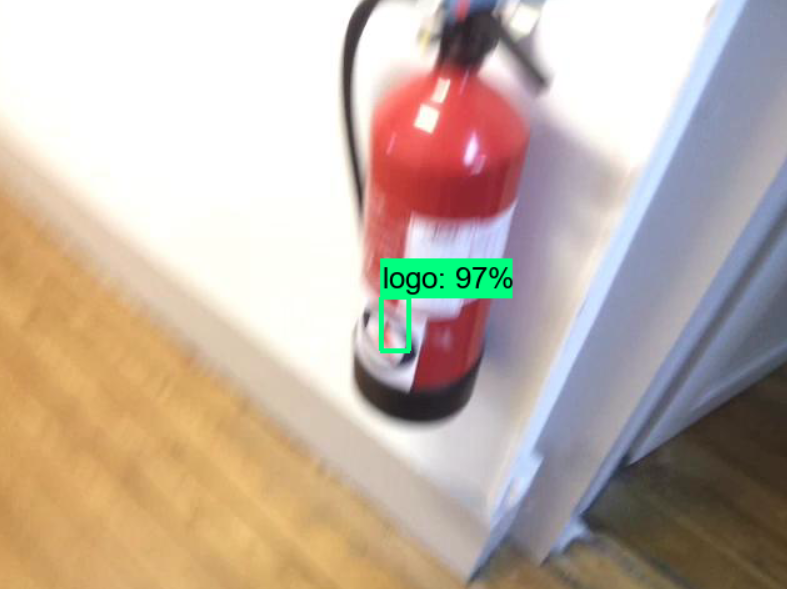
\includegraphics[width=4cm]{images/detection3.PNG}
	\end{subfigure}
	\begin{subfigure}[t]{4cm}
		\centering
		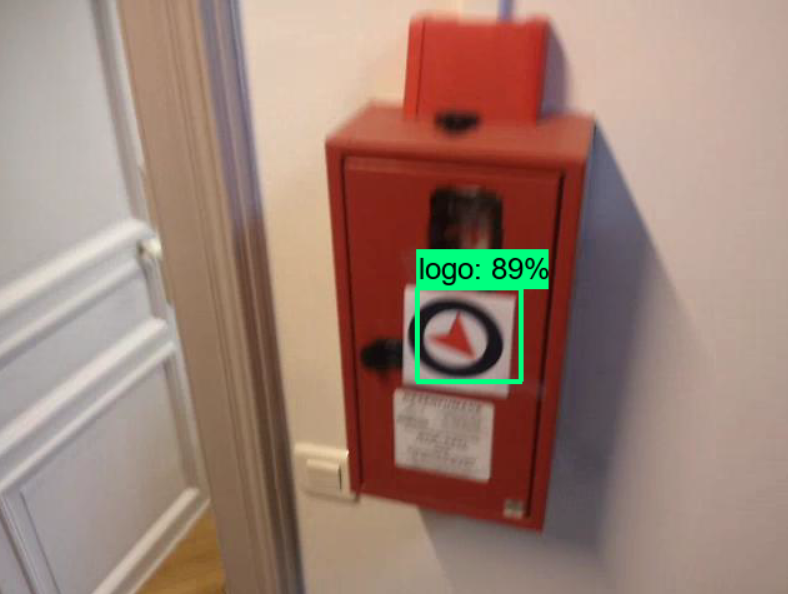
\includegraphics[width=4cm]{images/detection4.PNG}
	\end{subfigure}
	\caption{Sucessful predictions on test images.}\label{fig:predictionResult}
\end{figure}

\subsection{Back to computer vision}

\paragraph{}
The technics used are design in order to detect false positives from true positives. The edge detection and shape recognition cannot be used since blurry images may be real logos. That's why others arguments are used.

\subsubsection{Format}
\paragraph{}
This one is pretty straightforward; the logos should be a square or not too far from it depending on the angle of the camera. this allows to remove a few false positive that have a ratio height/width above $2$ or bellow $1/2$. This filter is quite fast to apply (the complexity is $\mathcal{O}(1)$)

\subsubsection{Color distribution}
\paragraph{}
One thing that hasn't been used so far is the color distribution. Indeed, all the logo images should have - if the image is not too blurry - a pic in the color distribution in blue, white and red. However, this is not always the case, especially when the camera is moving too fast and the luminosity is not good enough.


\captionsetup[subfigure]{labelformat=simple, labelsep=period}
\begin{figure}
	\centering
	\begin{subfigure}[t]{10cm}
		\centering
		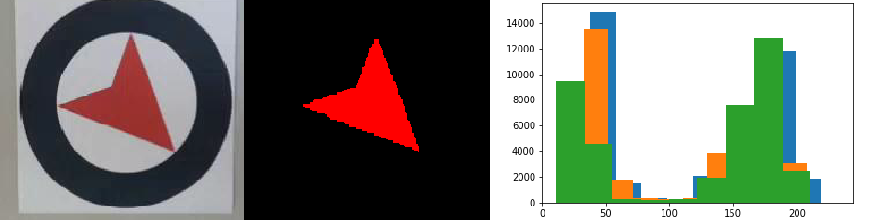
\includegraphics[width=9cm]{images/colorDistrib1.png}
		\caption{The distribution is neat, can be distinguished easily}
	\end{subfigure}
	\begin{subfigure}[t]{10cm}
		\centering
		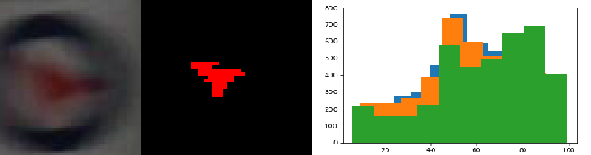
\includegraphics[width=9cm]{images/colorDistrib2.png}
		\caption{The distribution is more mixed; the amount of red remains effective.}
	\end{subfigure}
	\caption{Images with detection of red and the distribution of the colors.}\label{fig:colorDistrib}
\end{figure}

However, it is possible to try to detect the amount of red in the picture, with what is considered red quite permissive ($red > 40$ and $red > \max(2*green, 2*blue)$). Indeed, a positive image should have at least a little bit of red, but must not be more than a $25\%$ of the picture (number determined by using positive and negative samples, see \ref{fig:colorDistrib}).


\section{Next steps}

\subsection{Tracking}

\paragraph{}
The time factor is not used here. The frames are treated in an independent way, without any correlation nor order. A tracking algorithm could remedy this problem, such as using a K Nearest Neighbours Kalman filter \cite{kalman}. This method would use an already detected object, and try to follow the evolution from one frame to another. This is not trivial, since the camera is moving, the blurriness is definitely not helping the case.

\paragraph{}
The study of the trajectory could also be something used. Indeed, if we detect an object for a few frames, we can have an idea of where to look for coming up frame, and feeding the network with a restricted zone to identify the box (the normalization would be more effective that way). Extrapolating the position from a linear regression of the latest positions and cropping the image with a slightly bigger size than boxes previously detected could refine the new box detection.

\subsection{Offline Treatment}
\paragraph{}
If the treatment is done offline (or with a reasonable delay), knowing the "future" can really be useful in the detection of false positive and false negative. Indeed, an object not detected in between two frames where the object is can be recovered afterwards. The other way around, an object detected only for one frame with no continuity could be removed.

\subsection{Real time treatment}
\paragraph{}
The model used here does not allow the real time processing, at least on CPU. A few amelioration could improve this, such as jumping a few frames and extrapolating the position of the logos in the middle. Otherwise, lighter network could be used, such as the YOLO \cite{yolo} have better performances (reaching 45fps or 155fps for the light version); this is however always a trade off between speed and accuracy.

\begin{thebibliography}{9}
\bibitem{canny} 
John Canny. 
\textit{A Computational Approach to Edge Detection}. 
1986.

\bibitem{googleAPI}
Huang J, Rathod V, Sun C, Zhu M, Korattikara A, Fathi A, Fischer I, Wojna Z,
Song Y, Guadarrama S, Murphy K.
\textit{Speed/accuracy trade-offs for modern convolutional object detectors}.
2017.

\bibitem{nadam}
Timothy Dozat.
\textit{Incorporating Nesterov Momentum into Adam}.
2015.
 
\bibitem{kalman} 
Dan Iter, Jonathan Kuck, Philip Zhuang.
\textit{Target Tracking with Kalman Filtering, KNN and LSTMs}.
2016.

\bibitem{yolo}
Joseph Redmon, Santosh Divvala, Ross Girshick, Ali Farhadi.
\textit{You Only Look Once: Unified, Real-Time Object Detection}.
2016.
 
\bibitem{dataAugmentation}
Jason Wang; Luis Perez.
\textit{The Effectiveness of Data Augmentation in Image Classification using Deep Learning}.
2017.
 
\bibitem{interpretability}
Xuan Liu, Xiaoguang Wang, Stan Matwin.
\textit{Interpretable Deep Convolutional Neural Networks via Meta-learning}.
2018.

\bibitem{nasnet} 
Barret Zoph, Vijay Vasudevan, Jonathon Shlens, Quoc V. Le.
\textit{Learning Transferable Architectures for Scalable Image Recognition}.
2018.
\end{thebibliography}




\end{document}
